%Allgemein
\begin{wrapfigure}[23]{r}{.5\textwidth}
\vspace{-4.5em}
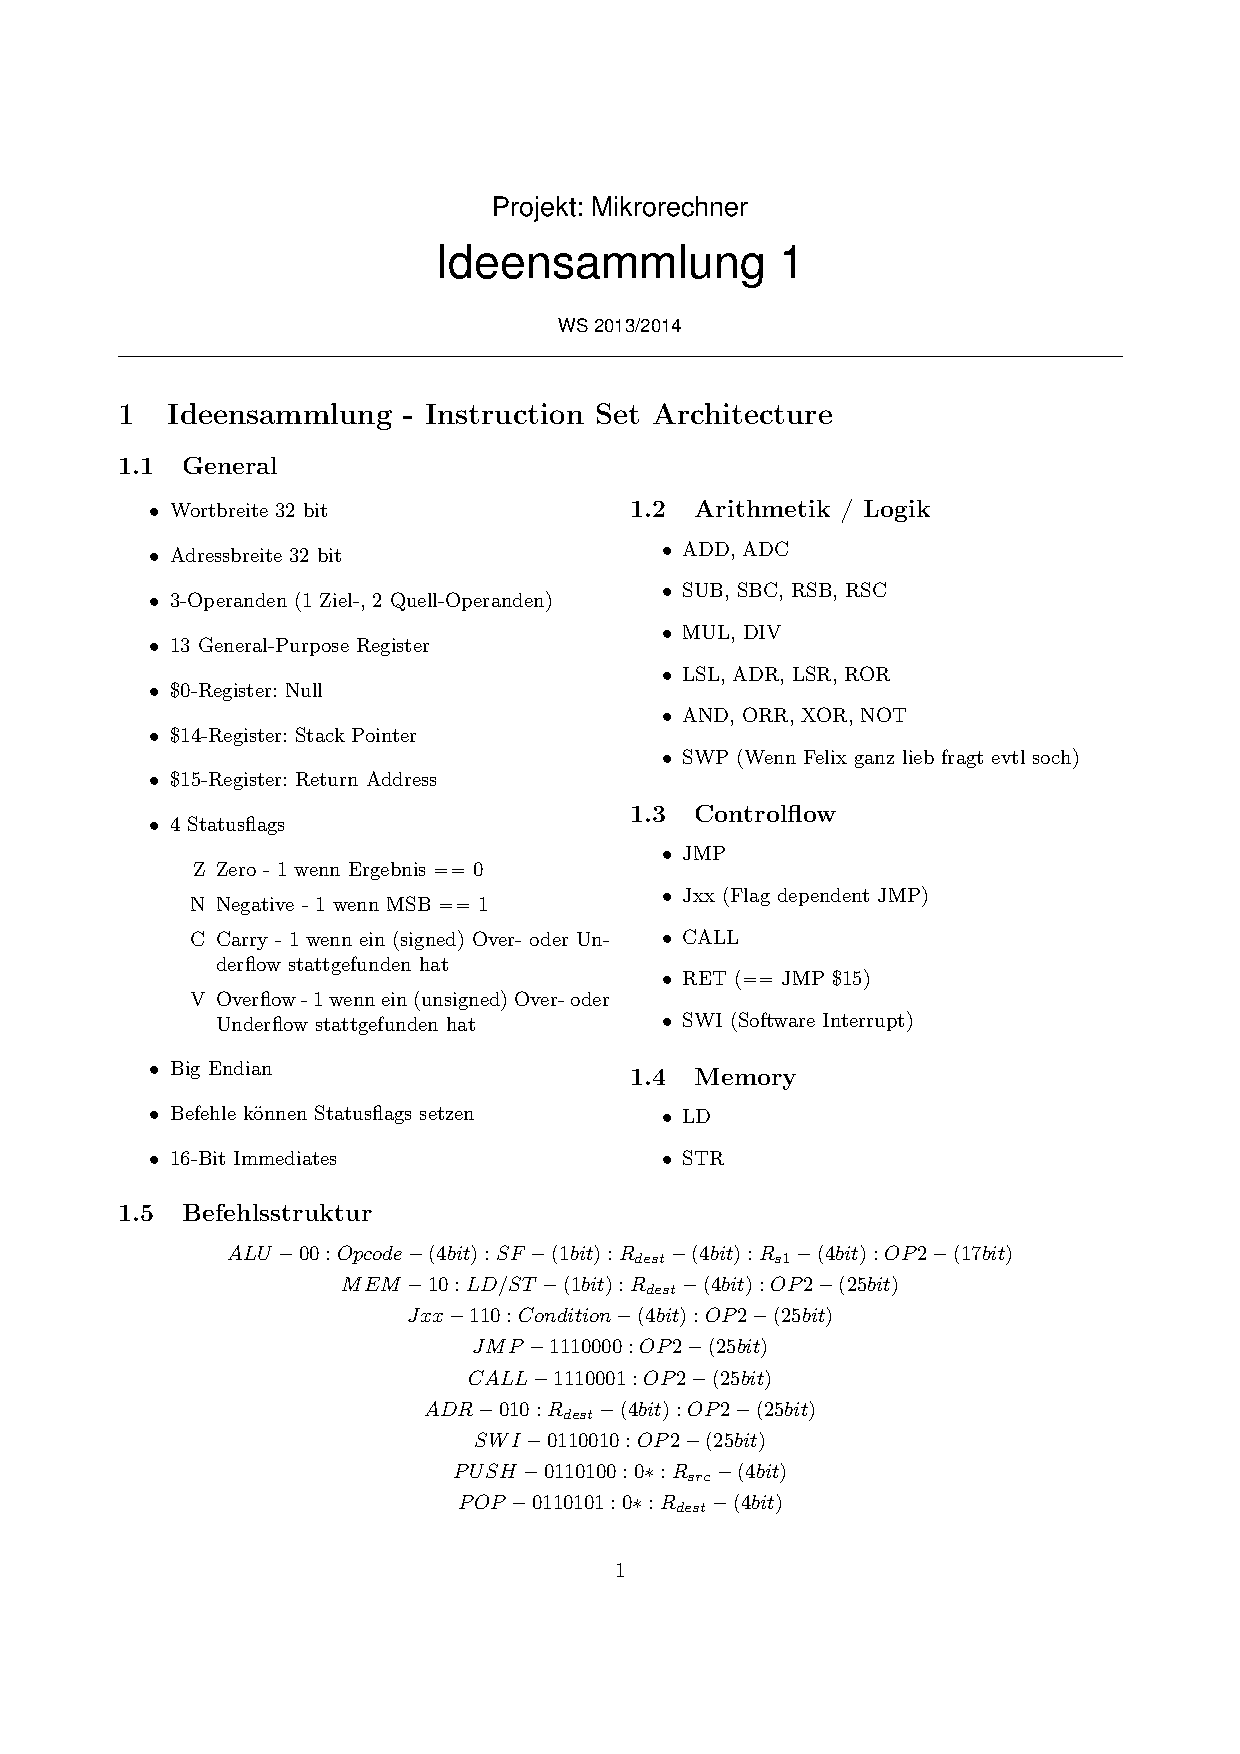
\includegraphics[width=.5\textwidth]{images/Ideensammlung.pdf}
\vspace{-4.5em}
\caption{\label{gen:Idee} Ideensammlung}
\end{wrapfigure}
Am 17. Oktober 2013 war der Startschuss der Veranstaltung. Die ersten Termine waren im Sinne der Wissensreaktivierung gestaltet. In mehreren Terminen wurden die grundlegenden Konzepte 
von Rechnerarchitekturen wiederholt, um Wissenslücken zu schließen und alle auf einen Stand zu bringen. Erst später ging die eigentliche Projektphase los.
Nach den Vorlesungsterminen ging es in die Gruppen. Jede Gruppe bestand aus 5-8 Personen. Unsere Gruppe bestand aus 5 Leuten und war damit die Kleinste. Ab diesem Zeitpunkt waren die Gruppen auf sich gestellt. Die Lehrkräfte waren nicht mehr für die Organisation zuständig, sondern hatten nur noch unterstützende und beratende Aufgaben.
In den ersten Wochen wurde noch nicht so viel Praktisches gemacht. Wir teilten uns zunächst in eine Hardware- und Softwaregruppe auf. Damit beide Teilgruppen an einem Strang ziehen, investierten wir die Zeit in den ersten Wochen für eine kleine Ideensammlung bezüglich unserer ISA und unserer Befehlsstruktur. \todo{ISA und Befehlsstruktur sind in etwa das gleiche. Hier bitte was anderes hinschreiben}
Es wurden Fragen grundlegende Fragen geklärt wie z.B. die Wort- und Adressbreite, Little oder Big Endian und wie unsere Befehlsstruktur aufgebaut ist. Ein Teil unserer Ideensammlung der ersten Wochen ist in der Abbildung \autoref{gen:Idee} zu sehen.

Um eine gute Kommunikation zu gewährleisten, trafen wir uns jeden Donnerstag am Informatikum. Wir arbeiteten alle in einem Raum, weil uns eine direkte Kommunikation wichtig war. Bei Problemen konnte so der direkte Kontakt hergestellt werden. Denn es stellte sich schnell raus, dass Abweichungen von der ersten Ideensammlung unumgänglich waren. So konnten Konflikte schnell diskutiert und beseitigt werden.

Darüber hinaus nutzten wir Git, um die Ergebnisse zusammenzutragen und alle auf einem Stand zu halten. Außerdem konnten so Fragen sofort geklärt werden und mussten nicht bis auf den nächsten Donnerstag verschoben werden.

\section{Warum Python} %Ortmann
In unserem Pojekt haben wir an vielfältigen Stellen auf die Sprache Python zurückgegriffen. Python wurde sowohl zu Modellierungsunterstüzung als auch zum Bau von Emulatoren und UIs verwendet. Diese waren zwar nicht zwingend relevant für das Abschließen des Projektes, erleichterten unsere Arbeit allerdings sehr. \newline
Die Entscheidung für die Sprache Python wurde in unserer Gruppe sehr früh getroffen. Schon beim ersten Treffen waren alle Gruppenmitgleider ausreichend über VHDL Vor- und vorallem Nachteile informiert, um eine Wrapper-Sprache ausprobieren zu wollen. Bereits beim ersten Treffen haben wir beschlossen, dass wir Python nicht nur nutzen wollen, weil die Sprache intuitiv ist, sondern weil wir ein Python Package fanden, dass den gesamten Hardware-Modellierungsprozess von VHDL auf Python Konstrukte abstrahieren konnte - MyHDL. Mit diesem Package konnte die Modellierungsarbeit und später auch die Verifikation erheblich erleichtert werden. MyHDL bildet eine Art Brücke zwischen den Eigenheiten der mit VHDL möglichen Prozessbeschreibung hin zu dem bekannten Pythonkonzept der Generatoren. Mit Pythons Unit Test Framework war es viel leichter den MyHDL Code zu testen, als tatsächliche Hardwaretests durchzuführen. Zumindest in den frühen Stadien des Projektes hat es einen großen Teil der Arbeit sehr erleichtert.

Abgesehen von dem Wrapper-Package MyHDL hat die Sprache Python noch an anderen Stellen viel Einfluss auf unser Projekt gehabt. Als erstes war ein Compiler für unseren eigenen Assembler wichtig. Wir wollten unsere Assembler Befehle in Bitcode übersetzen können. Dieser Assembler wurde in Python geschrieben und übersetzt alle Assemblerbefehlsworte in den Bitcode, wie er in userer zu dem Zeitpunkt jeweils aktuellen ISA spezifiziert war. Unsere endgültige ISA ist in \autoref{AP:ISA} zu finden. Mit dem Bitcode war allerdings noch nicht viel anzufangen, da die Hardwarespezifikation noch lange nicht fertig war. Folglich brauchten wir eine Möglichkeit, unsere Assemblerprogramme auf Gültigkeit zu testen, am besten sogar eine Ausführungsmöglichkeit. Es folgte ein weiteres kleines Unterprojekt in Python.

Wir haben uns zum Ziel gesetzt, einen Emulator zu schreiben, der den später modellierten Microcontroller vollständig widerspiegeln sollte. Damit wollten wir es uns ermöglichen, bereits kleine Programme in unserem eigenem Assembler-Code schreiben und ausprobieren zu können. Den Emulator haben wir ebenfalls in Python geschrieben, er emuliert analog zur HDL Hardwarestruktur eine CPU, eine RAM/ROM und einen Programmcode in der ROM. Auf dieser Ausführungseinheit fehlte nur noch die Introspektion, die wir brauchten, um den Ablauf der Programme zu verifizieren und auch Datenflüsse in der emulierten Hardware zu optimieren. Da wir den Emulator eng an die tatsächliche Hardwarespezifikation angelehnt haben, war es uns möglich das spätere Verhalten des Microcontrollers am Beispiel des Emulators zu beobachten und zu verbessern. Um also den nötigen Grad an Einsicht in unsere Programminterna zu erhalten, schrieben wir unsere eigene \glqq Emulator UI'', eine Art Debugger für Programm- und Hardwarezustände. Für das grafische Frontend des Emulators verwendeten wir das UI-Framework GTK für Python.

\section{Ein Wort zur Lizenz} %Ortmann
\textit{GPLv3, GNU General Public License version 3}\\
Von Beginn an haben wir unser Projekt weltöffentlich und zugänglich auf Github gemacht. Im Zuge dieser Art der Veröffentlichung erschien es uns nötig, den Code unter Lizenz zu stellen. Es gibt zu genau diesem Zweck viele verschiedene Arten von Lizenzen; viele haben den Zweck den tatsächlichen Autor des Codes davor zu schützen, dass Dritte diese Arbeit verkaufen und den Autor ausbeuten. Dabei darf jedoch nicht außer acht gelassen werden, dass der Code Open Source ist und jedem zugänglich sein \textit{soll}.

Wir haben uns in unserem Projekt für die Lizenz \textit{GNU General Public License version 3} entschieden. Damit sind vorallem die Nutzer unserer Software nicht benachteiligt, die Nutzung ist uneingeschränkt möglich und erlaubt. Der Download, das Verteilen und auch die Veränderung zu eigenen Zwecken werden in der Lizenz behandelt und explizit erlaubt. Was jedoch nicht erlaubt ist, ist die kommerzielle Distribution unseres Codes ohne uns als Autoren zu informieren und zu beteiligen. Es lässt sich festhalten, dass die Lizenzsierung hauptsächlich aus dem Wunsch heraus motiviert wurde, unseren Code nicht an einen unbekannten Dritten rechtlich zu verlieren.

\section{Werkzeuge}
\subsection{Git}
Git ist ein Versionskontrollsystem, dass das verteilte Arbeiten in Gruppen erleichtert. Weiterhin bietet git sehr gutes Source-Code-Magement. Anders als herkömmliche Versionierungssoftware, setzt git nicht auf die Existenz eines zentralen Servers und erfordert nicht zwingend Internetanbindung.
Für unser Projekt haben wir den kostenlosen git-Hoster \textit{github} genutzt. Hier ist auch unsere Projekthistorie in Form von Commits in das Projektrepository festgehalten.

\subsection{Pycharm}
% TODO

\subsection{Latex}
% TODO

\subsection{Altera}
Altera\footnote{\url{http://dl.altera.com/}} ist eine Entwicklungsumgebung für den FPGA. Es bietet sowohl Unterstüztung für das Programmieren mit VHDL/Verilog als auch das Überführen des Codes in eine lauffähige Version auf dem FPGA. Auch Debugging ist möglich, in dem man einzelne Leitungen überwachen und auswerten kann. Dies kam uns vor allem gegen Ende der Zeit, als wir auf der Hardware arbeiteten zu Gute. So wurde der eine oder andere Fehler im Code \glqq schnell\grqq \ entdeckt. 

\subsection{Hades}
Hades\footnote{\url{http://tams-www.informatik.uni-hamburg.de/applets/hades/webdemos/index.html}} ist eine in Java-Programmierte Digitale Schaltsimulation. Sie diente dazu unser Design anschaulich und verständlich zu machen. Man kann sehr gut die Vernetzung und das Zusammenspiel der einzelnen Komponenten sehen und nachvollziehen. Der fertige Schaltplan ist theoretisch in der Lage den Code auszuführen. Dies wurde aber nicht genutzt, denn es wurde ein eigener Emulator entwickelt, der effizienter war und unseren Bedürfnissen besser entspricht.

\subsection{Gtkwave}
Gtkwave\footnote{\url{http://gtkwave.sourceforge.net/}} wurde genutzt, um Komponenten und Verschaltungen des Myhdl-Codes zu evaluieren und zu debuggen. MyHdl ist in der Lage aus dem Code direkt eine VCD\footnote{\url{https://en.wikipedia.org/wiki/Value_change_dump}}-Datei zu erstellen, die von Gtkwave ausgelesen und dargestellt werden kann. So können Schaltverhalten und Fehler nachvollzogen und behandelt werden, ehe sie auf dem FGPA landen, wo die Fehler wesentlich schwieriger zu finden sind. Auch Timing-Probleme können hier erkannt und frühzeitig beseigt werden.
\begin{figure}[H]
\centering
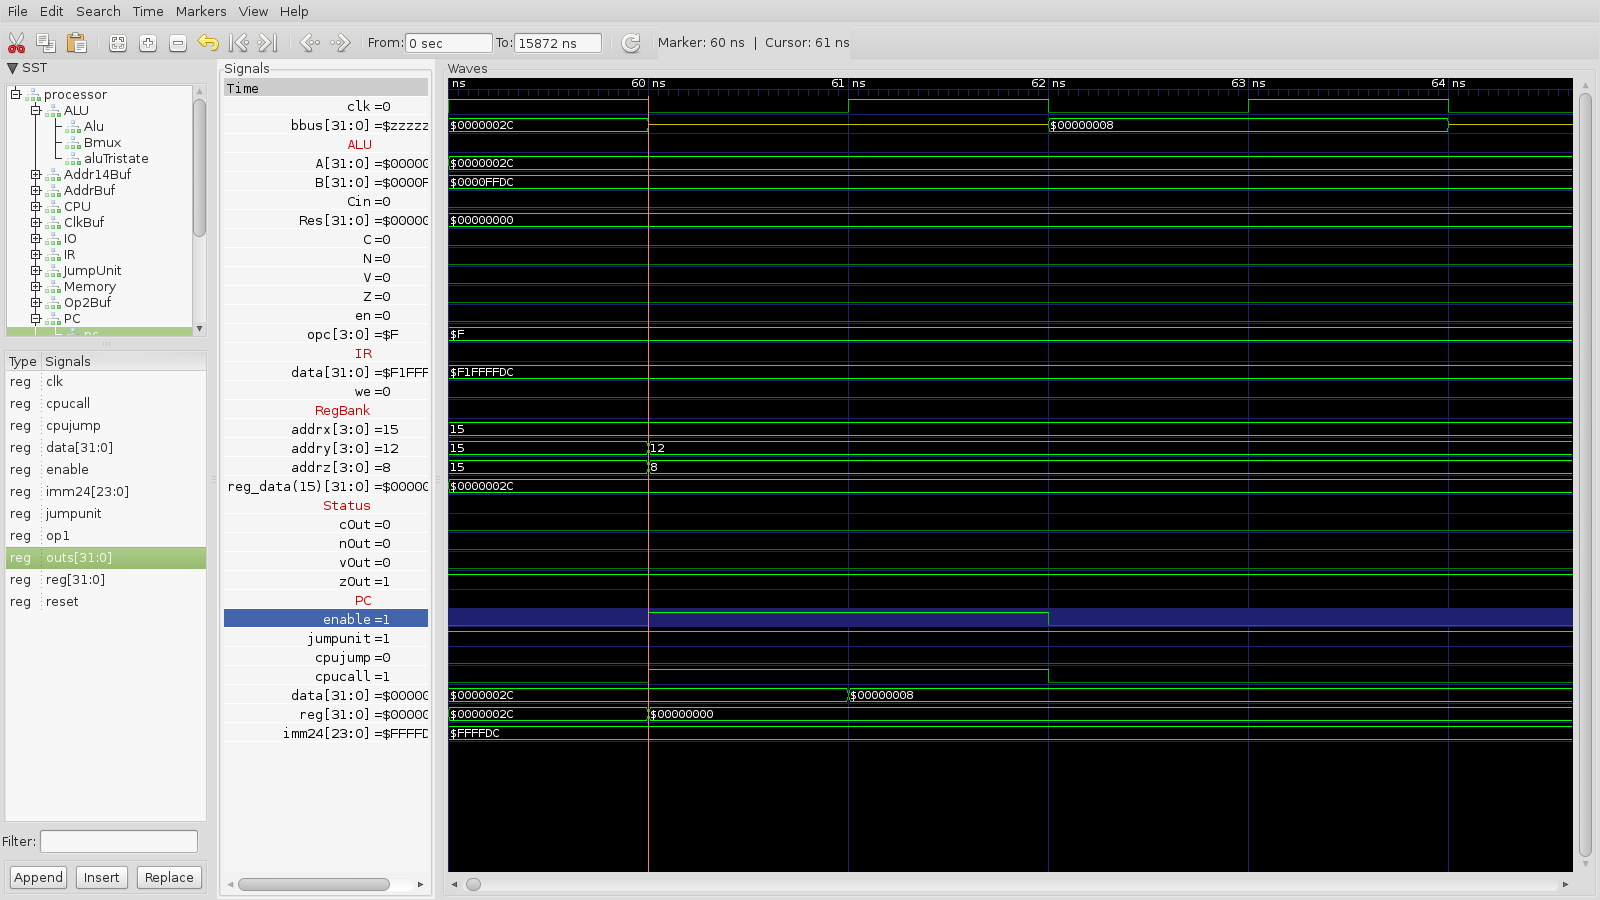
\includegraphics[width=\textwidth]{images/gtkwave.png}
\caption{\label{gen:gtkwave}Gtkwave}
\end{figure}

\section{Testen}
% TODO: unit testing
